\documentclass{beamer}
\usetheme[pageofpages=of,% String used between the current page and the
                         % total page count.
          bullet=circle,% Use circles instead of squares for bullets.
          titleline=true,% Show a line below the frame title.
          alternativetitlepage=true,% Use the fancy title page.
       %   titlepagelogo=logo-polito,% Logo for the first page.
       %   watermark=watermark-polito,% Watermark used in every page.
       %   watermarkheight=100px,% Height of the watermark.
       %   watermarkheightmult=4,% The watermark image is 4 times bigger
                                % than watermarkheight.
          ]{Torino}

\author{Brendon J. Brewer}
\title{Bayesian probability theory}
\institute{Department of Statistics, The University of Auckland}
\date{{\color{blue} https://www.stat.auckland.ac.nz/\~{ }brewer}\\
\vspace{10pt}
{\color{blue} @brendonbrewer}}

\begin{document}

\begin{frame}[t,plain]
\titlepage
\end{frame}

\begin{frame}[t]{Propositions}
Propositions are {\it statements that can be either true or false}.\\
Examples:\vspace{20pt}

$A$: {\small Hillary Clinton will be president of the USA on June 14th, 2017.}\\
$B$: {\small The current temperature in Auckland is greater than 14$^{\circ}$C.}\\
$C$: {\small $\Omega_\Lambda \neq 0$.}\\
$D$: {\small David Hogg has had more than 500 mg of caffeine today.}
\end{frame}

\begin{frame}[t]{Propositions}
Propositions can be {\it combined} to make others, using the operators
{\bf and} ($\wedge$), {\bf or} ($\vee$), and {\bf not} ($\neg$): \vspace{20pt}

$A \wedge B$\\
$C \vee A$\\
$\neg D$\\
$\neg (A \vee (C \wedge D))$
\end{frame}

\begin{frame}[t]{Notation}
The operator {\bf and} is sometimes denoted with a comma.\vspace{20pt}

\begin{equation}
(A \wedge B) \equiv (A, B)
\end{equation}

\end{frame}

\begin{frame}[t]{Quantifying propositions}
Science is largely concerned with the {\it plausibility} of propositions.
Plausibility depends on the information you have, so is a function of {\it
two} propositions. Examples:\vspace{20pt}

$P(A | B)$\\
$P(\neg D | (C \vee D))$\\
$P((C \wedge D) | \neg A)$\vspace{20pt}

Read the ``$|$'' as ``{\bf given}'' or ``{\bf conditional on}''.
\end{frame}


\begin{frame}[t]{Constraints on plausibility}
Some properties of plausibility:\vspace{20pt}

$P(A \vee B) \geq P(A)$\\
%$P(A \wedge B) \leq P(A)$\\
$P(A \vee (B \vee C)) = P((A \vee B) \vee C)$\vspace{20pt}

Where'd the RHS go? $|| D$
\end{frame}

\begin{frame}[t]{Constraints on plausibility}
Some properties of plausibility:\vspace{20pt}

$P(A \vee B) \geq P(A)$\\
$P(A \wedge B) \leq P(A)$\\
$P(A \vee (B \vee C)) = P((A \vee B) \vee C)$\vspace{20pt}

These imply the {\bf sum rule} and the {\bf product rule}, and hence that
{\bf plausibilities are probabilities}.
\end{frame}

\begin{frame}[t]{Sum and product rule\hspace{170pt}$|| C$}
$P(A \vee B) = P(A) + P(B) - P(A \wedge B)$\\
\vspace{20pt}
$P(A \wedge B) = P(A)P(B|A)$
\end{frame}

\begin{frame}[t]{Bayes' Rule\hspace{170pt}$|| I$}
Bayes' Rule (consequence of product rule and commutativity of {\bf and})
\begin{equation}
P(H | D) = \frac{P(H)P(D|H)}{P(D)}
\end{equation}
where\vspace{20pt}
$P(D) = P(H)P(D | H) + P(\neg H)P(D | \neg H)$
(consequence of sum rule)
\end{frame}

\begin{frame}[t]{Terminology\hspace{170pt}$|| I$}
\begin{equation}
P(H | D) = \frac{P(H)P(D|H)}{P(D)}
\end{equation}
\begin{equation}
\textnormal{(posterior probability)} =
\frac{\textnormal{(prior probability)}\times\textnormal{(likelihood)}}{\textnormal{(marginal likelihood)}}
\end{equation}
\end{frame}

\begin{frame}[t]{Another Bayes' Rule\hspace{170pt}$|| I$}
For $N$ mutually exclusive, exhaustive hypotheses
$H_1, H_2, ..., H_N$, we have $N$ posterior probabilities:

\begin{equation}
P(H_i | D) = \frac{P(H_i)P(D|H_i)}{P(D)}
\end{equation}

where
\begin{equation}
P(D) = \sum_{i=1}^N P(H_i)P(D|H_i)
\end{equation}
\end{frame}

\begin{frame}[t]{Another Bayes' Rule\hspace{170pt}$|| I$}

{\bf This is the most important form of Bayes' rule.}

\begin{equation}
P(H_i | D) = \frac{P(H_i)P(D|H_i)}{P(D)}
\end{equation}

where
\begin{equation}
P(D) = \sum_{i=1}^N P(H_i)P(D|H_i)
\end{equation}
\end{frame}


\begin{frame}[t]{Exercises!\hspace{170pt}$|| I$}
\end{frame}

\begin{frame}[t]{Parameter estimation}
In most applications, we can use the ``parameter estimation'' story. E.g.
Let $\theta$ be a quantity we want to know. Then the hypotheses might be:

\begin{eqnarray}
H_1 &\equiv& \theta = 5\\
H_2 &\equiv& \theta = 6\\
H_3 &\equiv& \theta = 7
\end{eqnarray}

The data could also be a number. E.g. the conditioning proposition could be
\begin{equation}
D = 4
\end{equation}

The previous version of Bayes' rule can be applied to each of the.
\end{frame}

\begin{frame}[t]{Parameter estimation}
Define the prior distribution $p(\theta)$


\begin{equation}
p(\theta | D) \propto p(\theta)p(D|\theta)
\end{equation}

This notation hides {\bf a lot}!
\end{frame}


\begin{frame}[t]{Ingredients I}
Bayesian inference need the following inputs:

\begin{itemize}
\setlength{\itemsep}{20pt}
\item A {\bf hypothesis space} describing the set of possible answers to our
question (``parameter space'' in fitting is the same concept).
\item A {\bf prior distribution} $p(\theta)$ describing how plausible
each of the possible solutions is, not taking into account the data.
\end{itemize}
\end{frame}

\begin{frame}[t]{Ingredients II}
Bayesian inference need the following inputs:
\begin{itemize}
\item A {\bf sampling distribution} $p(D | \theta)$ describing our knowledge
about the connection between the parameters and the data.
\end{itemize}

When $D$ is known,
this is a function of $\theta$ called the {\bf likelihood}.
\end{frame}


\begin{frame}[t]{The Posterior Distribution}
The data helps us by changing our prior distribution to the {\bf posterior
distribution}, given by
\begin{eqnarray*}
p(\theta | D) &=& \frac{p(\theta) p(D|\theta)}{p(D)}
\end{eqnarray*}
where the denominator is the normalisation constant, usually called either
the {\bf marginal likelihood} or the {\bf evidence}.
\begin{eqnarray*}
p(D) &=& \int p(\theta)p(D|\theta) \, d\theta.
\end{eqnarray*}

\end{frame}

\begin{frame}[t]{Posterior Distribution vs. Maximum Likelihood}
The practical difference between these two concepts is greater in higher
dimensional problems.
\begin{center}
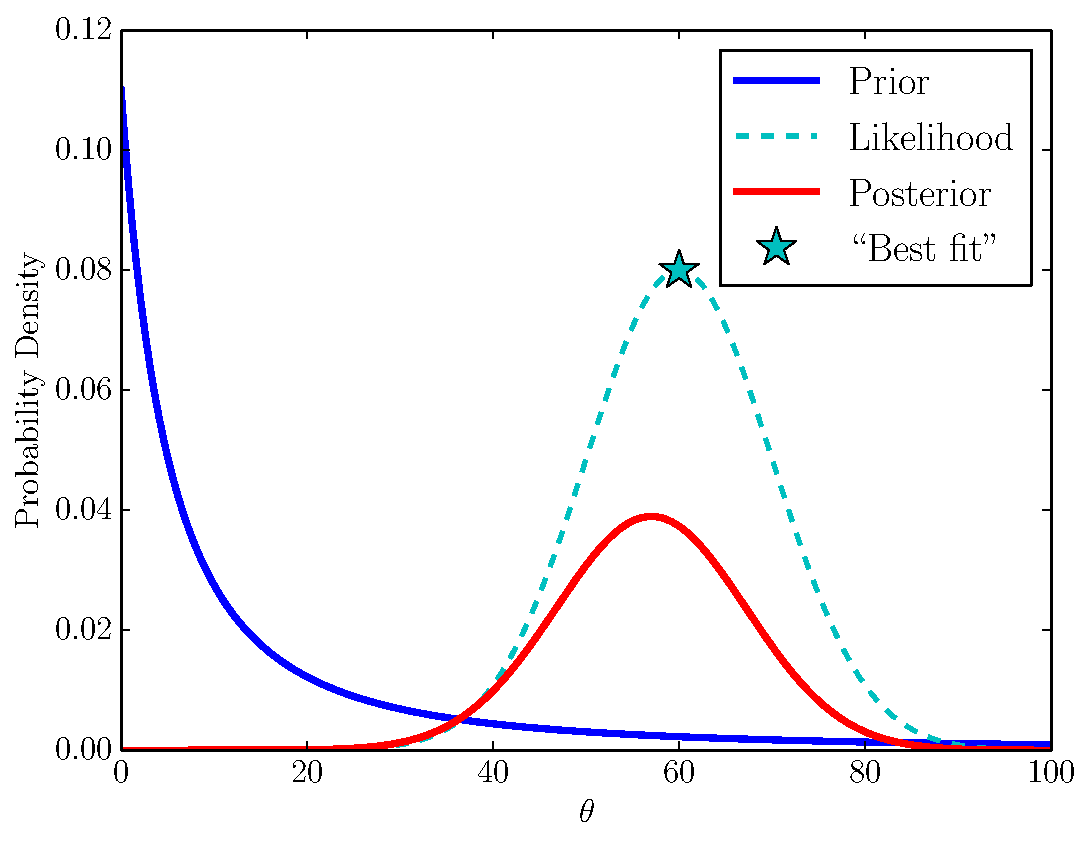
\includegraphics[scale=0.35]{bayes.pdf}
\end{center}
\end{frame}




\begin{frame}[t]{Updating Probabilities: Example}
\begin{center}
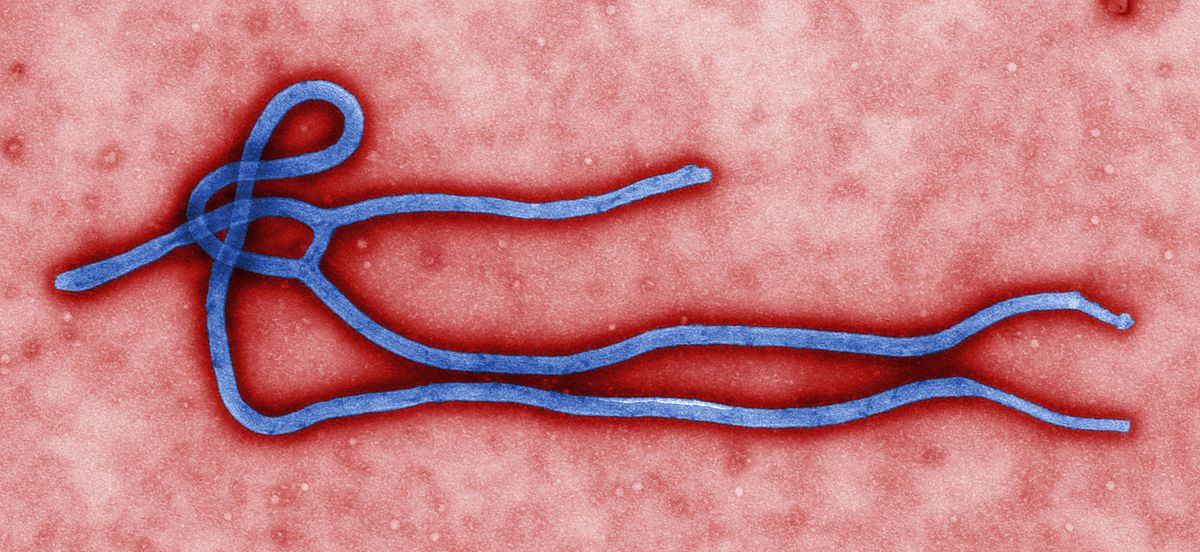
\includegraphics[scale=0.5]{ebola.jpg}
\end{center}
A patient goes to the doctor because he as a fever. Define
\begin{center}
\begin{tabular}{ll}
$H \equiv $ & ``The patient has Ebola''\\
$\neg H \equiv $ & ``The patient does not have Ebola''.
\end{tabular}
\end{center}

\end{frame}

\begin{frame}[t]{Updating Probabilities: Example}
Based on all of her knowledge, the doctor assigns probabilities to the two
hypotheses.
\begin{eqnarray*}
P(H) &=& 0.01\\
P(\neg H) &=& 0.99
\end{eqnarray*}

But she wants to test the patient to make sure.
\end{frame}



\begin{frame}[t]{Updating Probabilities: Example}
The patient is tested. Define

\begin{center}
\begin{tabular}{ll}
$D \equiv $ & ``The {\bf test says} the patient has Ebola''\\
$\neg D \equiv $ & ``The {\bf test says} the patient does not have Ebola''.
\end{tabular}
\end{center}

If the test were perfect, we'd have $P(D | H) = 1$, $P(\neg D | H) = 0$,
$P(D | \neg H) = 0$, and $P(\neg D | \neg H) = 1$.
\end{frame}


\begin{frame}[t]{Updating Probabilities: Example}
The Ebola test isn't perfect. Suppose there's a 5\% probability it simply gives
the wrong answer. Then we have:

\begin{eqnarray*}
P(D | H)   &=& 0.95\\
P(\neg D | H) &=& 0.05\\
P(D | \neg H)   &=& 0.05\\
P(\neg D | \neg H) &=& 0.95
\end{eqnarray*}

\end{frame}

\begin{frame}[t]{Updating Probabilities: Example}
Overall, there are four possibilities, considering whether the patient has
Ebola or not, and what the test says.

\begin{center}
$(H, D)$\\
$(\neg H, D)$\\
$(H, \neg D)$\\
$(\neg H, \neg D)$
\end{center}


\end{frame}

\begin{frame}[t]{Updating Probabilities: Example}
The probabilities for these four possibilities can be found using the product
rule.
\begin{eqnarray*}
P(H, D) &=& 0.01 \times 0.95\\
P(\neg H, D) &=& 0.99 \times 0.05\\
P(H, \neg D) &=& 0.01 \times 0.05\\
P(\neg H, \neg D) &=& 0.99 \times 0.95\\
\end{eqnarray*}
\vspace{-45pt}

These four possibilities are {\bf mutually exclusive} (only one of them is true)
and exhaustive (it's not ``something else''), so the probabilities add up to 1.

\end{frame}

\begin{frame}[t]{Updating Probabilities: Example}
The test results come back and say that the patient has Ebola. That is, we've
learned that $D$ is true. So we can confidently rule out those possibilities
where $D$ is false:

\begin{eqnarray*}
P(H, D) &=& 0.01 \times 0.95\\
P(\neg H, D) &=& 0.99 \times 0.05\\
{\color{red} P(H, \neg D)} &=& {\color{red} 0.01 \times 0.05}\\
{\color{red} P(\neg H, \neg D)} &=& {\color{red} 0.99 \times 0.95}\\
\end{eqnarray*}


\end{frame}


\begin{frame}[t]{Updating Probabilities: Example}
We are left with these two possibilities.

\begin{eqnarray*}
P(H, D) &=& 0.01 \times 0.95\\
P(\neg H, D) &=& 0.99 \times 0.05
\end{eqnarray*}

It would be strange to modify these probabilities just because we deleted the
other two. The only thing we have to do is renormalise them, by dividing by the total, so they sum to 1 again.
\end{frame}

\begin{frame}[t]{Updating Probabilities: Example}
Normalising, we get

\begin{eqnarray*}
P(H | D) &=& (0.01 \times 0.95)/(0.01 \times 0.95 + 0.99\times0.05) = 0.161\\
P(\neg H | D) &=& (0.99 \times 0.05)/(0.01 \times 0.95 + 0.99\times0.05) = 0.839
\end{eqnarray*}
\end{frame}

\begin{frame}[t]{Moral}
Bayesian updating is completely equivalent to:
\begin{itemize}
\item Writing a list of possible answers to your question
\item Giving a probability to each
\item Deleting the ones that you discover are false.
\end{itemize}

It just seems more complicated than this because we often apply it to more
complex sets of hypotheses.
\end{frame}



\end{document}

